\documentclass[format=acmtog]{acmart}
\usepackage{graphicx}
\graphicspath{ {./img/} }

\begin{document}
\title{Movement Model for Motion Matching}

\maketitle

\section{meta}
We have a movement model. It is flexible both and parameter count and values.

We have reference motion. It is flexible under warping.

We want a fit between these two.

\subsection{Ideas for fitting optimizations}
Could we start by distributing user control changes in animation frames ?

\section{Introduction}
Realistic and responsive character animation is important for establishing immersion in computer games. The complexity of human movement makes it difficult to construct such an experience by hand. Instead we record reference data using motion capture and construct animation synthesizers that either stitches clips together, samples inferred statistical models, or learns control policies for a physical model and mimics the animations. Recent advances 
%in both industry and research communities 
show a strong tendency towards complex closed systems guided by weak control signals. Notably \citep{holden.ea20} and \citep{Bergamin19} uses a spring-damper system due to \citep{kermse.04} for a motion matching system, while \citep{startke20} generate control trajectories by upsampling an unspecified smooth user input using a neural network. In \citep{zhang18} an interpolation between current and desired direction is fed directly to a generative model and in \citep{peng17} a physical model is trained to follow randomly generated paths by allowing a 2 meter divergence. \kenny{Our work use XXX? or is similar to YYY? or ?}

To our best knowledge it has not been investigated how to construct and synchronize weak control signals to animation synthesizers for full body locomotion. This is important for computer games. It is an industry standard in AAA productions to have a gameplay layer that controls changes to character position and a separate animation layer that tries to generate animations that matches the changes in positions \citep{holden18}. We suggest the term \textit{movement model} to describe the gameplay layer logic that controls character position in response to player input. In game productions the movement model is carefully tuned by designers to give a response that \textit{feels appealing}, it is used to predict future character movement and even for analyzing the validity of game levels. These industry practices poses requirements to how we construct our movement models. 

The movement model seems an ideal control signal for animation synthesizers. We have a history of movement available and can integrate the model for predictions.Hence, the movement model is both a weak signal and describes the actual movement of game characters and this introduce a challenge. If there is a disconnect between the movement model and the animation synthesizer output, we might allow the animations to diverge from the movement model and later catch up. But this severely impacts the types of game experiences that can be created as we loose exact positioning of our character and it changes the feeling of movement in response to player input which is critical for immersion \magnus{(REF)}. If we enforce synchronization between the two layers artifacts such as foot sliding and a general degradation of realism and quality kick in. It is an industry standard to carefully synchronize animations and movement models by hand at great economical cost to avoid these issues. \changed{We show how current best practice compared to our method in Figure \ref{fig:teaser}.}

%We propose that it is a valuable effort to investigate movement models and suggest a procedure to do so. It is a task that runs parallel to the more researched area of modeling full body kinematics, and has stricter requirements for simplicity as models should be extremely fast to evaluate and open for manual tweaks to get the feeling of movement just right. 
We propose to investigate movement models as a valuable mechanism for handling both weak control and actual motion description. In order to be applicable in AAA game production the models are required to be simple, as automated as possible to avoid unnecessary manual labour, extremely fast to evaluate, and open for manual artistic tweaks to change the feeling of movement if needed.

In the following pages we introduce a method for composing movement models from primitives that can be automatically fitted to reference animations using auto differentiation. We suggest a model composition for plane locomotion and show procedures to simplify and align the animations to avoid modeling complex and unnecessary details while preserving visual quality. Our modeling task is ill-posed since in the limit player input could contain complex low level control signals similar to what is found in the animations, which would greatly reduce requirements to the model as the control signal would itself represent what we are trying to model. We regularize the task by using the novel concept of \textit{control genomes} to formalize the reduction of low level control input to high level signals corresponding better to expected player behavior. Finally we present a procedure to determine movement in animations from foot contact analysis which was discovered as a side effect of our work and can be used in its own right.



\section{Basic terminology}
Define animation database as $\mathcal{D}$

Define Movement model

Define Animation warping.

\section{Related work}
\subsection{Animation Warping}
Animation warping can be viewed as a generative model trained on $D$. 


\section{Movement Model}
A movement model describes how an entity moves through space given control input. It consists of internal parameters such as velocities and accelerations. Control input could be a direction of movement supplied by a human using a gamepad, or longer paths supplied by a game engine AI system.

We have not seen any formal description of the movement model. Ususally some ad hoc newtonian physics concepts are combined with springs and animation curves to control the system.

In the following we limit the description to locomotion in the plane. 

We parameterize the movement model as $\mathcal{M}=L,T$ where $L=l_0 \ldots l_n$ is a set of locomotion modes and $T=t_0 \ldots t_m$ is a set of transition types between locomotion modes. A movement model defines the behaviour of an actor $\mathcal{A}=\boldsymbol{\omega},p,\dot{p},r,\dot{r}$ where $p$ and $r$ describe position, orientation and their derivatives.  $\boldsymbol{\omega}=\omega_0 \ldots \omega_n$ contains contribution weights for $l \in \mathcal{L}$. Notice $||\vec{\boldsymbol{\omega}}||^2=1$ and usually only a couple of modes will be active as in a transition between walking and running where $\boldsymbol{\omega}=\omega_{walk}:0.8, \omega_{run}:{0.2}, \omega_{other}:0$

An actor is moved with a control signal $\mathcal{C}=l_c,\Delta{t}_c, p_c,r_c$ containing locomotion mode, timestep and target position and orientation. The sparsity of the control signal ilustrates an inherent uncertainty in character animation, as we are challenged to infer a detailed path of movement through often complex environements given a very limited disambiguation or hints to the desired trajectory [Holden A deep learning ...]. We notice that a sampling of the immediate sorroundings could potentially be added as part of the control signal as in [Holden pfnn]. A step of the actor state can be described as two seperate functions.
\begin{equation}
\begin{split}
p^*,r^*&=step(\mathcal{A},\mathcal{L}, \mathcal{C})\\
\boldsymbol{\omega}^*&=step_{\omega}(\boldsymbol{\omega},\mathcal{T}, \Delta{t}_c)
\end{split}j
\end{equation}
MISSING: We need to keep track of an transition value [0,1]. For $step_{\omega}$ to keep the transitions continuous in $\Delta{t}_c$ each $t\in\mathcal{T}$ should define a mapping from $\Delta{t}$ to a normalized interpolation value which also describes the duration of that transition. Each individual $t$ can be modelled uniquely or in a unified approach, using animator supplied curves, sigmoids, linear interpolation or even a neural network to capture more subtleties in the transitions. In the case of transitions that are interrupted, we simply freeze existing transitions, and perform the incoming transition as a weighted combination of multiple transitions. See fig. \ref{fig:frozen-transition}. By freezing and combining transition in the case of interruptions, we are effectively approximating unsampled areas of the locomotion mode manifold by interpolations. This could be avoided by expading $\mathcal{T}$ to also contain transition between combination of locomotion mode, or by expanding $\mathcal{L}$ for a wider sampling of the manifold.  
\begin{figure*}
  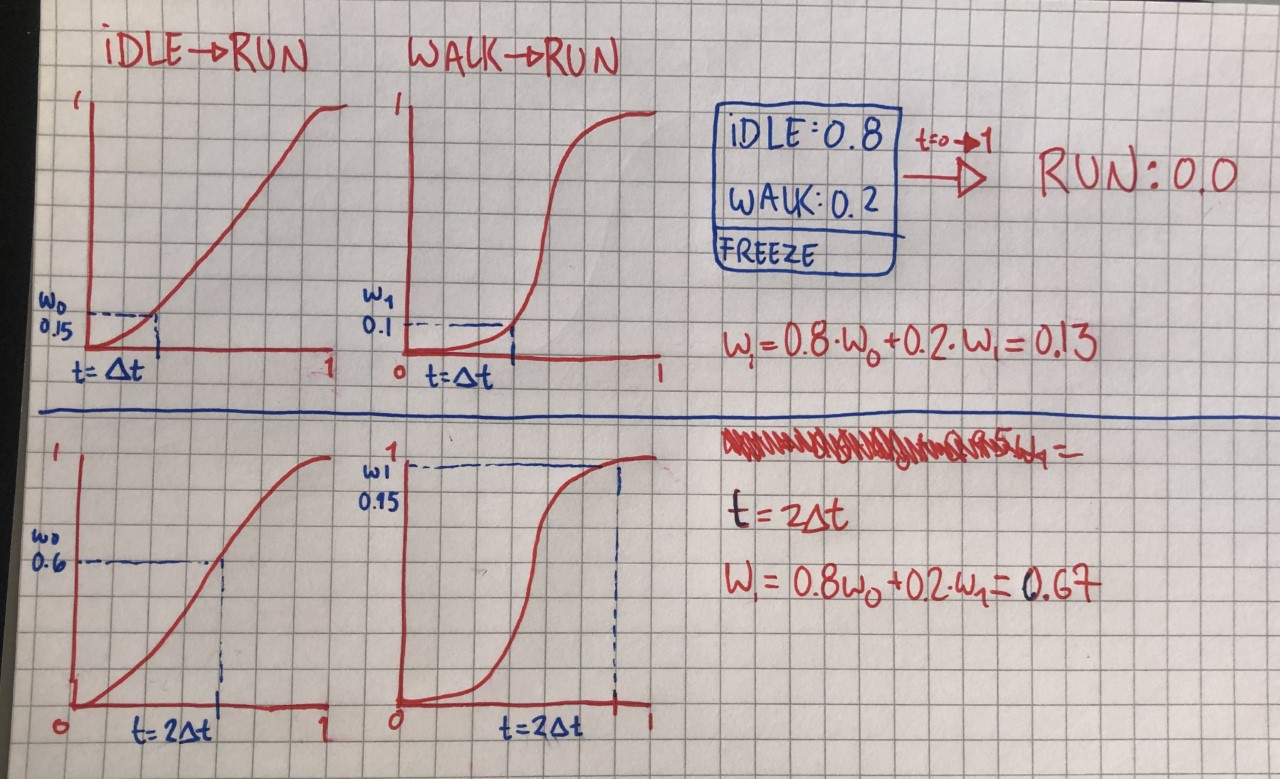
\includegraphics[width=\textwidth]{frozen-transitions}
  \caption{Frozen transition}
  \label{fig:frozen-transition}
\end{figure*}


Updates to the model is handled by the integration routine $p^*,q^*=I(m,C,p,q)$, and all $m_i,m_j\in\mathcal{M}$ are associated with a transition curve used to update $\vec{m}^*=T(C,\vec{m})$, ie., the update that handles transition times between movement modes. 
Each mode is associated with internal update procedures
\begin{equation}
\begin{split}
    p^*&=P(p,p',q')\\
    q^*&=Q(q,q',p')\\
\end{split}
\end{equation}
The update up the model is determined by the contribution of each movement mode in 
\begin{equation}
\begin{split}
    p^*&=\sum_{m\in{M}}{P_m*\vec{m}_m}\\
    q^*&=\sum_{m\in{M}}{Q_m*\vec{m}_m}\\
\end{split}
\end{equation}

Missing: Parameters exposed by P and Q update functions
Missing: Updates to velocities
Missing: Clear description of entire parameter set
Missing: Control signal could also contain

Notice that the formulation for $D$ is generic. In production a mapping between the generic movement model and a more context specific model would usually be needed. 

\subsection{missing}
Add animator constraint to model ? Example is 180. We dont start moving backwards immediately. First we rotate 90 degrees on the spot and then we start a 90 degree run to idle movement

Show very clear example. Pseudo code with idle and walk state. 

\section{Animation Warping}
We need a warping system that preserves ground truth. And some linear metric for divergence than can be scaled up from 0.


\section{Optimization Procedure}
We need some regularization to ill posed problem
\subsection{Primary movement modes}
Idea: Identify areas in the animations with cyclic movement for some duration. Cluster these segments into buckets with some threshold. We now have the velocity and number of main movement modes.
\subsection{Sparse user input}
If we allow extremely high frequency changes in the user input a wide variety of movement model configurations could follow the animation trajectory. We distribute sparse changes in user input over the animations, ie. few keypoints where we identify changes in the user input.

\section{Experiments}
Use precise movement model for other data driven system such as pfnn,. 

\bibliography{movement-model-for-motion-matching}{}
\bibliographystyle{plain}
\end{document}
